
\begin{exercise}
% !TEX root = ../main.tex


\pt{10}Een verticaal vallende steen legt in de laatste seconde, voor hij de grond bereikt, \SI{100}{m} af. Men veronderstelt dat hij vanuit rust vertrok.
\begin{enumerate}
\item Bepaal de snelheid op het ogenblik dat hij de grond bereikt.
\item Bepaal de hoogte vanwaar de steen viel en de tijd die hij daarvoor nodig had.
\end{enumerate}

\begin{oplossing}
%\footnote{$v=\frac{x_2-x_1}{t_2-t_1}+\frac{1}{2}g(t_2-t_1)=\frac{\Delta x}{\Delta t}+\frac{1}{2}g\Delta t$
%\newline
%$t_2=\frac{v_2}{g}=\frac{\Delta t}{2}+\frac{\Delta x}{g\Delta t}$, $x=\frac{1}{2}gt^2=\frac{1}{2g}\left(\frac{\Delta x}{\Delta t}\right)^2+\frac{\Delta x}{2}+\frac{g(\Delta t)^2}{8}$}
\item[\textit{gegeven}]$\Delta t=1,0\rm\,s$; $\Delta x=100\rm\,m$; $v_0=0$
\item[\textit{gevraagd}]$v_2$, $x_2$, $t_2$
\item[\textit{oplossing}]
\begin{enumerate}
\item 
\begin{minipage}[t]{.7\textwidth}
We kiezen de $x$-as naar beneden zodat de versnelling de valversnelling is, $a=g$. Als we $x_1$ beschouwen als de beginpositie van de beweging die de steen uitvoert in de laatste honderd meter, kunnen we de snelheid vinden waarmee de steen hieraan `begint'.
\begin{eqnarray*}
&&\Delta x=v_1\Delta t+\frac{1}{2}g\Delta t^2\\
&\Leftrightarrow&v_1=\frac{\Delta x-\frac{1}{2}g\Delta t^2}{\Delta t}
\end{eqnarray*}
\end{minipage}
\begin{minipage}[t][4.5cm][b]{.3\textwidth}
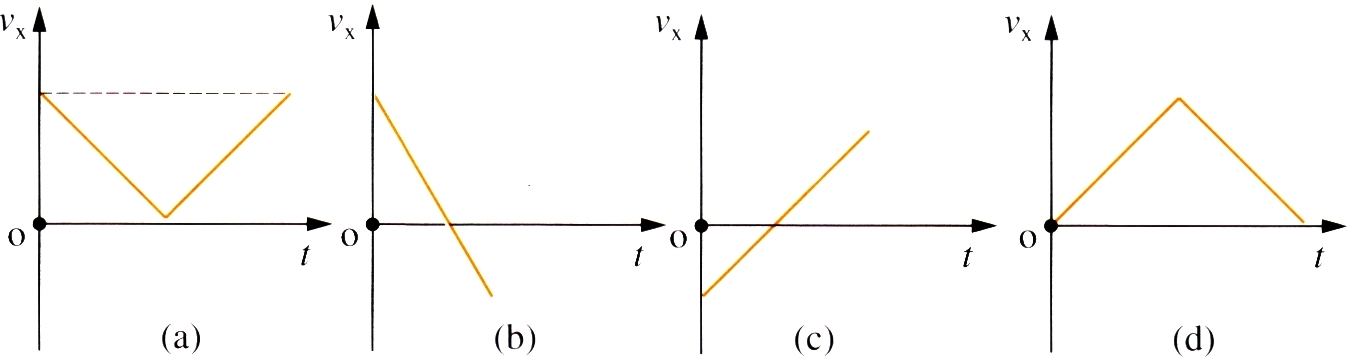
\includegraphics[height=6cm]{valbeweging}
\end{minipage}
\newline
\newline
\newline
Met de formule voor de snelheid van een EVRB, vinden we de snelheid op het einde van het interval.
\begin{eqnarray*}
v_2&=&v_1+g\Delta t\\
&=&\frac{\Delta x-\frac{1}{2}g\Delta t^2}{\Delta t}+g\Delta t\\
&=&\cdots\\
&=&\overline{v}+g\frac{\Delta t}{2}\\
&=&\SI{105}{m/s}
\end{eqnarray*}
Je kan dit ook afleiden door gebruik te maken van de formule voor gemiddelde snelheid, $\overline{v}=\frac{v_1+v_2}{2}$.
\item Omdat we de snelheid kennen, kunnen we de tijd vinden die de steen nodig heeft gehad om aan deze snelheid te komen. Vervolgens vinden we dan ook de afstand.
\begin{eqnarray*}
t_2=\frac{v_2}{g}=\frac{\overline{v}}{g}+\frac{\Delta t}{2}=\SI{10,7}{s}\\
x_2=\frac{1}{2}gt_2^2=\SI{561}{m}
\end{eqnarray*}
\end{enumerate}
\end{oplossing}

\end{exercise}
